\documentclass{article}
\usepackage{geometry}
\geometry{letterpaper, left=20mm, top=20mm, right=20mm, bottom=20mm}

\usepackage{graphicx}
\usepackage{amsmath}
\usepackage{listings}
\usepackage{xcolor}
\usepackage{hyperref}

\lstset{
    basicstyle=\ttfamily\small,
    breaklines=true,
    keywordstyle=\color{blue},
    commentstyle=\color{green!50!black},
    stringstyle=\color{red},
    frame=single,
    numbers=left,
    numberstyle=\tiny\color{gray}
}

\begin{document}

\noindent \textbf{Name:} Natalie Poche \\
\textbf{Date:} \today \\
\textbf{UFID:} 1533-4992

\begin{center}
    \large\textbf{Report 4 - Embedded Drivers and Bubble Level Application}
\end{center}

\section{Introduction}
This lab explores embedded systems development on the Raspberry Pi RP2040 microcontroller utilizing the Adafruit Feather RP2040 paired with a Propmaker FeatherWing. The primary objective is to design, implement, and integrate modular C++ driver libraries for an onboard LIS3DH I2C accelerometer and a WS2812 RGB NeoMatrix (64 addressable LEDs). Furthermore, an interactive bubble level application (\texttt{level.cpp}) is built on top of these drivers to demonstrate real-time sensor data acquisition and hardware actuation.

\section{Design}
The system architecture divides software responsibilities into three primary components:
\begin{enumerate}
    \item \textbf{LIS3DH Driver (\texttt{lis3dh.cpp / .h}):} Interfaces with the LIS3DH accelerometer over I2C1 (SDA on GPIO2, SCL on GPIO3) at 400\,kHz. It verifies communication via the \texttt{WHO\_AM\_I} register (expecting \texttt{0x33}), configures normal power mode at 1.34\,kHz ODR, and sets a $\pm 2\text{g}$ high-resolution range.
    \item \textbf{NeoMatrix Driver (\texttt{neomatrix.cpp / .h}):} Controls the $8 \times 8$ WS2812 LED matrix using RP2040 Programmable I/O (PIO) running an asynchronous one-wire protocol (\texttt{ws2812.pio}). It also drives GPIO\,10 high to enable power on the Propmaker FeatherWing NeoPixel port and handles serpentine pixel mapping.
    \item \textbf{Bubble Level Application (\texttt{level.cpp}):} Continuously samples acceleration values $(x, y, z)$. When both $|x| \le 0.1\text{g}$ and $|y| \le 0.1\text{g}$, it illuminates the center 4 LEDs in solid green. Otherwise, it lights up a single red LED indicating the direction of tilt.
\end{enumerate}

\begin{figure}[!ht]
    \centering
    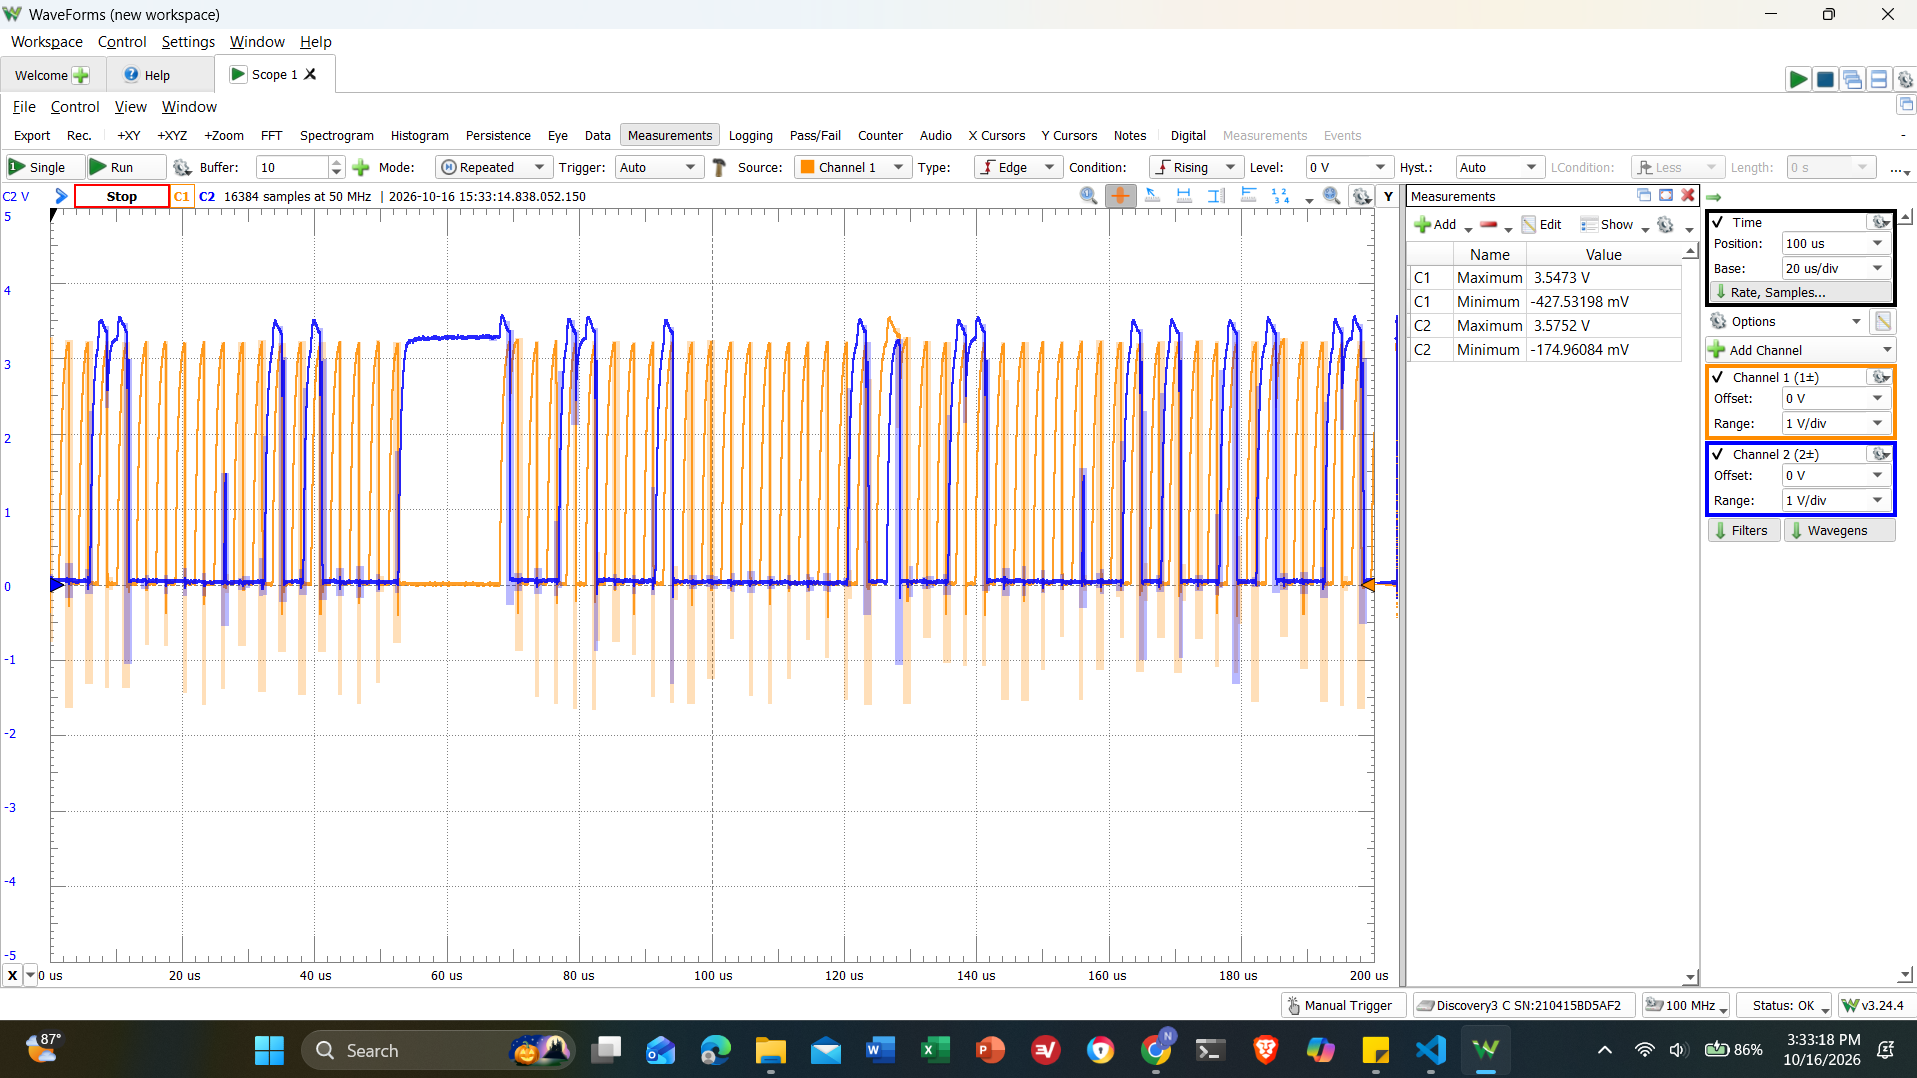
\includegraphics[width=0.7\linewidth]{img/i2c.png}
    \caption{Oscilloscope capture of the I2C bus showing synchronous two-wire serial communication between the RP2040 microcontroller and the LIS3DH accelerometer at a 400 kHz bus clock frequency. Channel 2 (blue) displays the clock line ($\text{SCL}$, GPIO 3) providing regular timing pulses, while Channel 1 (orange) displays the data line ($\text{SDA}$, GPIO 2). The visible bursts correspond to data transactions, such as addressing the accelerometer (\texttt{0x18}) and reading/writing internal configuration and data registers (e.g., polling \texttt{WHO\_AM\_I} or pulling axis measurements via \texttt{accel.update()}).}
    \label{fig:i2c_wave}
\end{figure}

\begin{figure}[!ht]
    \centering
    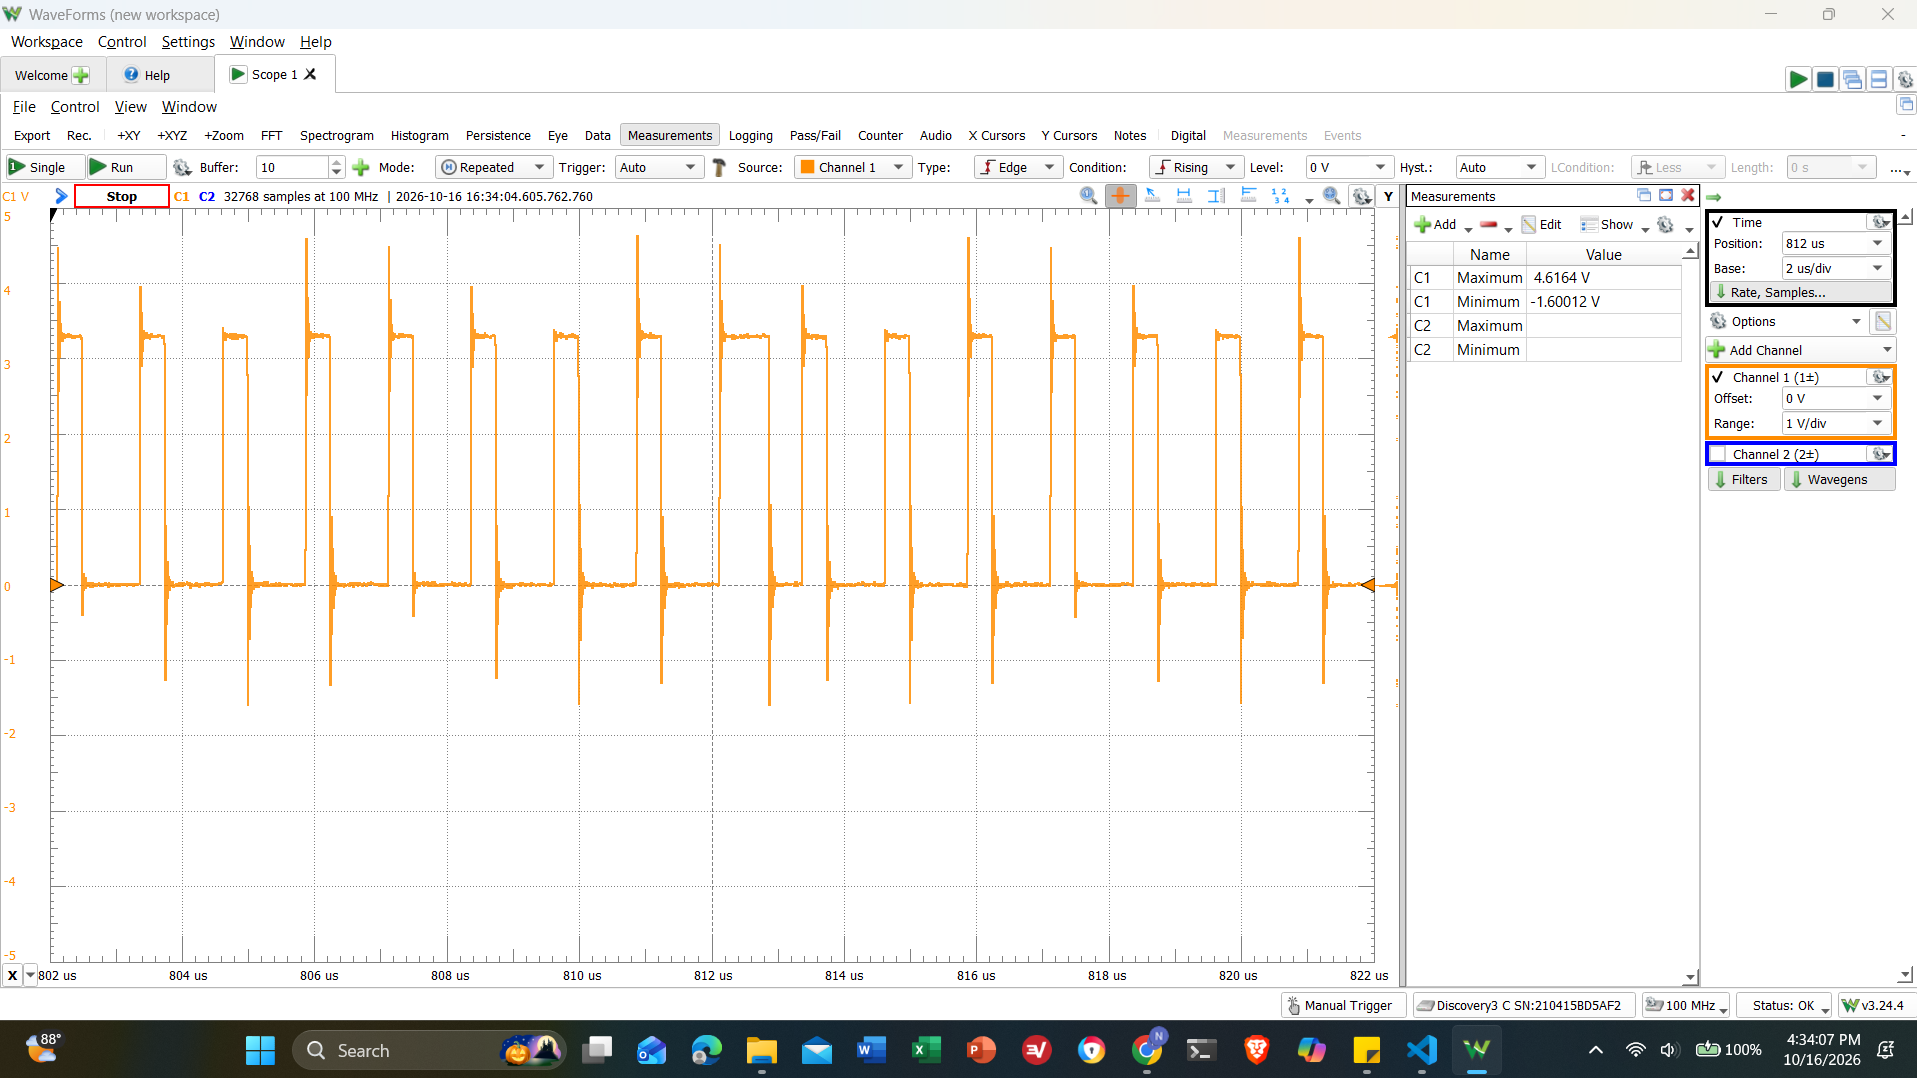
\includegraphics[width=0.7\linewidth]{img/neomatrix.png}
    \caption{Oscilloscope capture of the NeoMatrix output line implementing a strict single-wire timing protocol used to drive WS2812 RGB LEDs. Generated via the RP2040's Programmable I/O (PIO) state machine on GPIO 7 at 800 kHz, the waveform uses asymmetric pulse-width modulation where each high-frequency pulse encodes binary data based on precise duration timings ($T_1$, $T_2$, $T_3$). The repeated packet trains represent 24-bit GRB color frames shifted out sequentially to update all 64 pixels in the matrix buffer.}
    \label{fig:neomatrix_wave}
\end{figure}

\subsection{Theoretical Calculations}
In high-resolution mode with a $\pm 2\text{g}$ scale, the LIS3DH output data is 16-bit left-justified. The raw register values are shifted right by 6 bits (divided by 64), yielding a sensitivity of $4\text{ mg/digit}$ ($0.004\text{ g/digit}$). The gravitational acceleration along each axis is calculated as:

\[ a_x = \text{raw}_x \times 0.004\text{ g} \]
\[ a_y = \text{raw}_y \times 0.004\text{ g} \]
\[ a_z = \text{raw}_z \times 0.004\text{ g} \]

\section{Results and Discussion}
The bubble level application was successfully compiled into \texttt{level.uf2} using CMake and Ninja, and flashed onto the Adafruit Feather RP2040 via the UF2 bootloader.

\begin{table}[ht]
    \centering
    \caption{Comparison of Physical Orientation vs. Expected NeoMatrix Output}
    \begin{tabular}{|c|c|c|c|}
        \hline
        Orientation State & Measured $x$ (g) & Measured $y$ (g) & NeoMatrix Output \\
        \hline
        Flat (Level) & $0.02$ & $-0.01$ & Center 4 LEDs Green ($[3,3], [3,4], [4,3], [4,4]$) \\
        Tilted Right & $+0.45$ & $0.05$ & Single Red LED at Column 7 \\
        Tilted Forward & $-0.03$ & $-0.52$ & Single Red LED at Row 0 \\
        \hline
    \end{tabular}
    \label{tab:results}
\end{table}

\subsection{Implementation Challenges and Solutions}
\begin{itemize}
    \item \textbf{Windows Path Length Limitations:} Nesting projects deep within user directories caused CMake builds of native tools like \texttt{pioasm} to fail due to Windows 260-character path limits. \textit{Solution:} Migrated project directories to a short path root (\texttt{C:\textbackslash pico\_projects}).
    \item \textbf{Propmaker Power Control:} Initially, the NeoMatrix remained dark despite correct PIO initialization. \textit{Solution:} Configured GPIO\,10 as an output and drove it high to enable power on the Propmaker FeatherWing NeoPixel power rail. Also corrected GND and Power from feather to neomatrix as lab instructions say Black is goes to GND and Red goes to 5V, but it's switched.
\end{itemize}

\subsection{Suggestions for Improvement}
Structuring the drivers as standalone CMake library targets improves reusability across future embedded projects. Future enhancements could include adding DMA (Direct Memory Access) transfers to the NeoMatrix driver to reduce CPU overhead during pixel buffer writes.

\section{Conclusion}
The experimental results closely aligned with theoretical expectations (Table \ref{tab:results}). The LIS3DH accelerometer accurately reported tilt vectors, and the WS2812 PIO driver correctly updated the NeoMatrix display. Despite initial build toolchain and path configuration challenges, the project successfully demonstrated embedded driver abstraction and hardware integration on the RP2040 platform.

\newpage
\appendix
\section{Source Code Listings}

\subsection{\texttt{README.md}}
\lstinputlisting[language={}, caption={Project README and Build Instructions}]{embedded_driver/README.md}

\subsection{\texttt{CMakeLists.txt}}
\lstinputlisting[language=CMake, caption={CMake Configuration File}]{embedded_driver/CMakeLists.txt}

\subsection{\texttt{src/ws2812.pio}}
\lstinputlisting[language={[x86masm]Assembler}, caption={WS2812 PIO Assembly Program}]{embedded_driver/src/ws2812.pio}

\subsection{\texttt{src/level.cpp}}
\lstinputlisting[language=C++, caption={Bubble Level Application Main Source Code}]{embedded_driver/src/level.cpp}

\subsection{\texttt{src/lis3dh.h}}
\lstinputlisting[language=C++, caption={LIS3DH Accelerometer Driver Header}]{embedded_driver/src/lis3dh.h}

\subsection{\texttt{src/lis3dh.cpp}}
\lstinputlisting[language=C++, caption={LIS3DH Accelerometer Driver Implementation}]{embedded_driver/src/lis3dh.cpp}

\subsection{\texttt{src/neomatrix.h}}
\lstinputlisting[language=C++, caption={NeoMatrix Display Driver Header}]{embedded_driver/src/neomatrix.h}

\subsection{\texttt{src/neomatrix.cpp}}
\lstinputlisting[language=C++, caption={NeoMatrix Display Driver Implementation}]{embedded_driver/src/neomatrix.cpp}

\end{document}